\PassOptionsToPackage{ukrainian,english}{babel}
\documentclass[twocolumn]{el-author}

%\usepackage[...]{...}      This has been commented out as we are not using any additional packages here.  On the whole, they should be unnecessary.
\usepackage{mathtext}
\usepackage[T1,T2A]{fontenc}
\usepackage[english,ukrainian]{babel}
\usepackage{hyperref}
\usepackage{graphicx} %package to manage images
\usepackage[a4paper, total={7in, 9.5in}]{geometry}
\usepackage{makecell}
\graphicspath{ {images/} }
\newcommand{\hH}{\hat{H}}
\newcommand{\D}{^\dagger}
\newcommand{\ua}{\uparrow}
\newcommand{\nc}{\newcommand}
\renewcommand\theadfont{\normalsize\scshape}
\nc{\da}{\downarrow} \nc{\hc}{\hat{c}} \nc{\hS}{\hat{S}}
\nc{\bra}{\langle} \nc{\ket}{\rangle} \nc{\eq}{equation (\ref}
\nc{\h}{\hat} \nc{\hT}{\h{T}}\nc{\be}{\begin{eqnarray}}
\nc{\ee}{\end{eqnarray}}\nc{\rd}{\textrm{d}}\nc{\e}{eqnarray}\nc{\hR}{\hat{R}}\nc{\Tr}{\mathrm{Tr}}
\nc{\tS}{\tilde{S}}\nc{\tr}{\mathrm{tr}}\nc{\8}{\infty}\nc{\lgs}{\bra\ua,\phi|}\nc{\rgs}{|\ua,\phi\ket}
\nc{\hU}{\hat{U}}\nc{\lfs}{\bra\phi|}\nc{\rfs}{|\phi\ket}\nc{\hZ}{\hat{Z}}\nc{\hd}{\hat{d}}\nc{\mD}{\mathcal{D}}
\nc{\bd}{\bar{d}}\nc{\bc}{\bar{c}}\nc{\mc}{\mathcal}\nc{\ea}{eqnarray}\nc{\mG}{\mathcal{G}}\nc{\bce}{\begin{center}}
\nc{\ece}{\end{center}}
\date{20 Грудня 2018}

\begin{document}

\title{Вивчення закономірностей у спектрі водню і визначення сталої Рідберга}

\author{Сергій Поліщук}

\maketitle

\section{Мета роботи}

дослідження спектру випромінювання атомарного водню.

\section{Прилади і матеріали}

монохроматор УМ-2, ртутна лампа, воднева
газорозрядна трубка, джерело високої напруги для
живлення газорозрядної трубки, таблиця основних
довжин хвиль парів ртуті.

\section{Завдання}

\begin{enumerate}
	\item при домашній підготовці:
	\begin{itemize}
		\item  користуючись рекомендованою літературою, вивчити
закономірності випромінювання атома водню;
		\item  з фізичного практикуму записати хід роботи та будову і
принцип дії необхідних приладів;
		\item  зарисувати оптичну схему монохроматора УМ-2.
	\end{itemize}
	\item при виконанні роботи:
	\begin{itemize}
		\item  скласти електричну схему і показати її викладачеві для
перевірки;
		\item  за спектром випромінювання ртуті  проградуювати
монохроматор;
		\item  за спектром випромінювання водню визначити сталу
Рідберга;
		\item  виконати необхідні розрахунки з визначення шуканої
величини та можливих похибок;
		\item  оформити звіт і подати його викладачеві.
	\end{itemize}
	
\end{enumerate}

\section{Правила техніки безпеки}

\begin{itemize}
	\item  бережіться пошкодження очей, ні у якому разі не дивіться
назустріч випромінюванню ртутної лампи ;
	\item  при складанні електричної з схеми використовуйте
провідники з непошкодженою ізоляцією;
\end{itemize}

\section{Теоретичні відомості та опис установки}

Досліджуючи спектральний склад випромінювання атомарного водню
Й.~Бальмер показав (1885 р.), що спектральні лінії у видимій області
розташовані в строгому порядку. Пізніше (1913 р.) Н.~Бор, виходячи з
планетарної моделі атома Е.~Резерфорда, для пояснення спектральних
закономірностей водню постулює:

\begin{enumerate}
	\item Атом може перебувати лише в певних станах, у яких він,
усупереч класичній електродинаміці, не випромінює світло. Ці
стани називаються стаціонарними.
	\item Випромінювання відбувається, по-перше, квантами і, по-друге,
під час переходу атома із стаціонарного стану з вищою енергією
$E_{m}$ у стаціонарний стан з меншою енергією $E_{n}$. Тобто

\begin{equation} \label{eq:1}
hv = E_{m} - E_{n}
\end{equation}

	\item Стаціонарними слід вважати тільки ті орбіти, момент кількості
руху електрона на яких відповідає співвідношенню

\begin{equation} \label{eq:2}
m_{e}V_{r} = n \frac{h}{2 \pi}
\end{equation}

де $m_{e}$ - маса електрона, $V$ і $r$ - швидкість і радіус орбіти
електрона, $n$ - головне квантове число, яке може мати значення 1, 2, 3, 4...
\end{enumerate}

Обертовий рух електрона навколо ядра, згідно другого закону
Ньютона, описується формулою

\begin{equation} \label{eq:3}
m_{e} \frac{V^{2}}{r} = \frac{e^{2}}{4 \pi \varepsilon _{0} r ^{2}}
\end{equation}

Розв'язуючи рівняння (\ref{eq:2}) і (\ref{eq:3}) відносно $r$, знаходимо

\begin{equation} \label{eq:4}
r = \frac{h ^{2} \varepsilon _{0}}{\pi e ^{2} m _{e}}n^{2}
\end{equation}

Приведені вище міркування справедливі не лише для атома водню, а й для
воднеподібних іонів, заряд ядра яких $Ze$. Тоді рівняння (\ref{eq:4}) 
набуде вигляду:

\begin{equation} \label{eq:5}
r = \frac{h ^{2} \varepsilon _{0}}{Z \pi e ^{2} m _{e}}n^{2}
\end{equation}

Визначимо енергію електрона, що обертається навколо ядра. Його
повна енергія:

\begin{equation} 
E = E_{k} + E_{n} = \frac{m_{e} V^{2}}{2} 
+ \frac{Ze(-e)}{4 \pi \varepsilon _{0} r} = 
\frac{m_{e} V ^{2}}{2} - 
\frac{Ze^{2}}{4 \pi \varepsilon _{0} r}
\end{equation}

Підставивши в останнє рівняння значення $mV2$ з (\ref{eq:3}), одержимо

\begin{equation} 
E = - \frac{Ze^{2}}{8 \pi \varepsilon _{0} r}
\end{equation}

або з врахуванням (\ref{eq:5}):

\begin{equation} \label{eq:6}
E = - \frac{Z^{2} e^{4} m_{e}}{8h^{2} \varepsilon _{0}^{2}} \cdot \frac{1}{n^{2}}
\end{equation}

З (\ref{eq:6}) слідує, що енергія електрона в атомі квантована. Чим більше $n$,
тобто чим далі електрон від ядра, тим більшу енергію має атом. Під час
переходу атома із стаціонарного стану з вищою енергією
$E_{m} (m=n+1, n+2, n+3...)$ у стаціонарний стан з нижчою енергією $E_{n}$
відбувається випромінювання фотона $hv$. Тобто, на основі (\ref{eq:1}), одержуємо:

\begin{equation} 
hv = - \frac{Z^{2}e^{4}m_{e}}{8h^{2} \varepsilon _{0}^{2}} \cdot
\frac{1}{m^{2}} - 
\left ( - \frac{Z^{2}e^{4}m_{e}}{8h^{2} \varepsilon _{0}^{2}} \cdot \frac{1}{n^{2}} \right )
\end{equation}

або

\begin{equation} 
hv = - \frac{Z^{2}e^{4}m_{e}}{8h^{2} \varepsilon _{0}^{2}} 
\left ( \frac{1}{n^{2}} - \frac{1}{m^{2}} \right )
\end{equation}

Звідки

\begin{equation} \label{eq:7}
v = - \frac{Z^{2}e^{4}m_{e}}{8h^{3} \varepsilon _{0}^{2}} 
\left ( \frac{1}{n^{2}} - \frac{1}{m^{2}} \right )
\end{equation}

Коефіцієнт $\frac{e^{4} m_{e}}{8h^{3} \varepsilon _{0}^{2}} = 3.2896 \cdot 10^{15}c^{-1}$ одержав назву сталої Рідберга R.

Тоді

\begin{equation} 
v = Z^{2}R
\left ( \frac{1}{n^{2}} - \frac{1}{m^{2}} \right )
\end{equation}

Або

\begin{equation} \label{eq:8}
\lambda = \frac{c}{Z^{2}R \left ( \frac{1}{n^{2}} - \frac{1}{m^{2}} \right )}
\end{equation}

Якщо $n$ взяти рівним одиниці, а значить $m$ може мати значення 2, 3, 4,
5, то одержимо сукупність спектральних ліній, кожній з яких відповідає,
згідно (\ref{eq:8}), своя довжина хвилі. Множину цих ліній називають
спектральною серією. Комбінуючи подібним чином $n$ і $m$, одержують набір
серій, деякі характеристики яких наведені в таблиці \ref{tab:1}.


Спостереження спектрів у даній роботі виконується за допомогою
монохроматора УМ-2. Попередньо його необхідно проградуювати, тобто
встановити відповідність між поділками барабану монохроматора і
довжиною хвилі. З цією метою використовують стандартні спектральні лінії
ртуті, довжини хвиль для яких добре відомі. Вони зведені у таблицю \ref{tab:2}. У
цій таблиці наведені кольори спектральних ліній ртуті та відповідні їм
довжини хвиль.

\begin{table}[ht]
\caption{\label{tab:2} Стандартні спектральні лінії ртуті}
{\begin{tabular}{|l|l|}\hline
\thead{Колір лінії ртуті } & 
\thead{Довжина хвилі, нм}\\\hline
Червоний             & 623.4 \\\hline
Червоно - оранжевий  & 612.4 \\\hline
Червоно - оранжевий  & 607.3 \\\hline
Жовтий (ліва лінія)  & 579.1 \\\hline
Жовтий (права лінія) & 577.0 \\\hline
Жовто - зелений      & 546.1 \\\hline
Зелений              & 491.6 \\\hline
Синій                & 435.8 \\\hline
Синій                & 433.9 \\\hline
Синьо - фіолетовий   & 410.8 \\\hline
Фіолетовий           & 407.7 \\\hline
\end{tabular}}{}
\end{table}

\begin{figure}[ht]
\centering{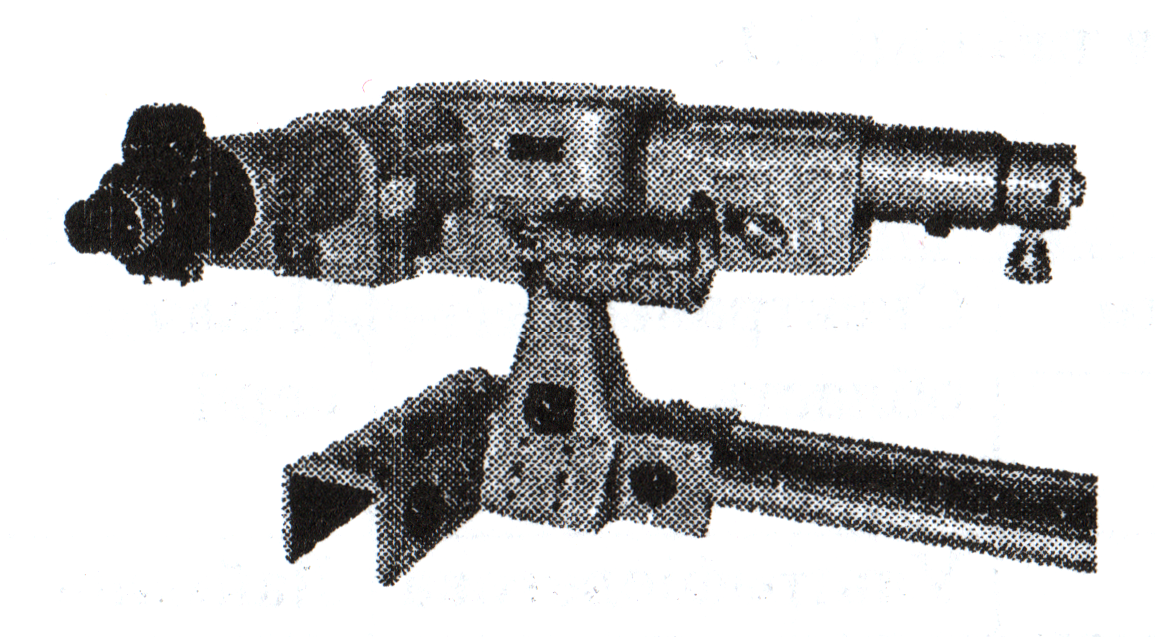
\includegraphics[width=80mm]{img_1}}
\caption{\source{} Зовнішній вигляд універсального монохроматора УМ-2}
\label{img:1}
\end{figure}

\begin{figure}[ht]
\centering{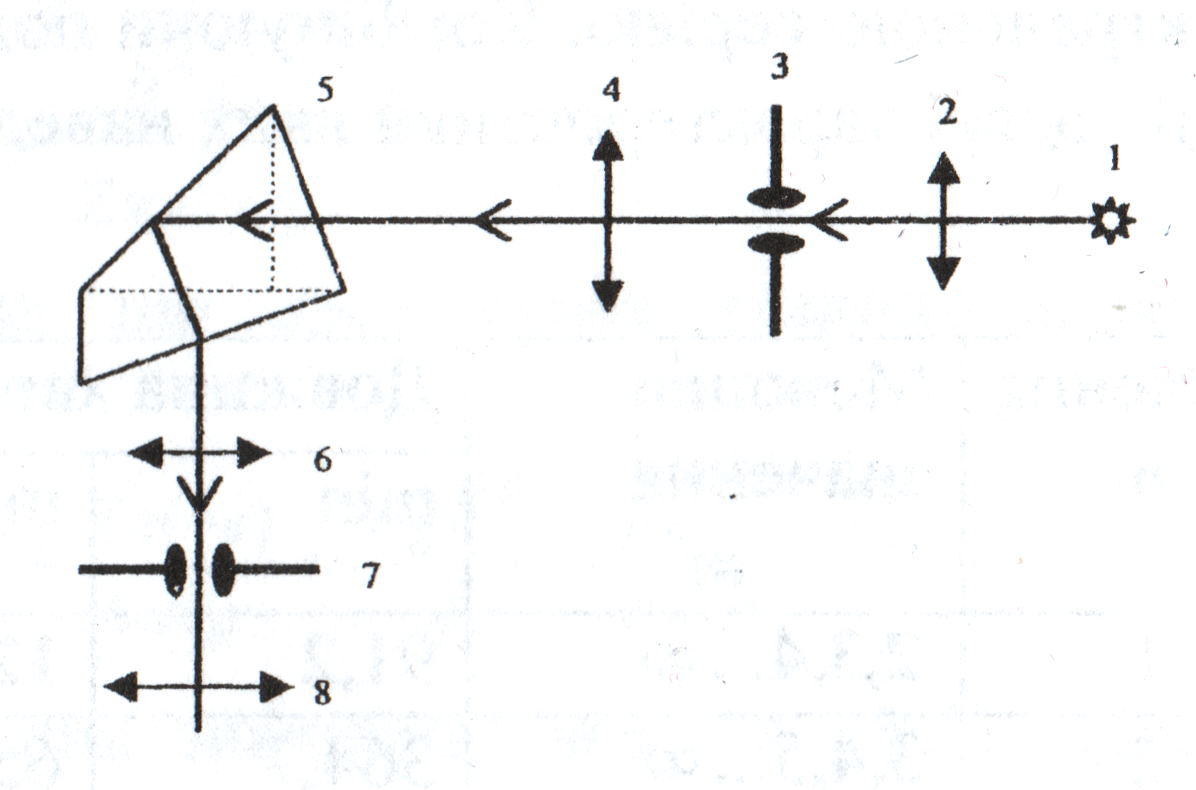
\includegraphics[width=80mm]{img_2}}
\caption{\source{} Оптична схема універсального монохроматора УМ-2}
\label{img:2}
\end{figure}

Світло від джерела 1 спрямовується на коліматорну вхідну лінзу 2,
освітлює щілину 3, яка розташована у фокусі об'єктивної лінзи коліматора 4,
і паралельним пучком потрапляє на збірну диспергуючу призму Аббе 5, яка
розкладає світло у спектр. Об'єктив 6, щілина 7 і окуляр 8 утворюють зорову
трубу.

Призма обертається механізмом, з'єднаним з барабаном, який має
спіральну шкалу з поділками від 0 до 3500$0$. При повороті барабана на одну
поділку система призм обертається на 20".


\section{Послідовність виконання роботи}

\begin{enumerate}
	\item На місце джерела світла встановити ртутну лампу. Домогтися
рівномірного освітлення лінзи 2.
	\item За допомогою щілини та окуляра домогтися чіткого і різкого
зображення однієї із спектральних ліній ртуті.
	\item Обертаючи барабан, послідовно, починаючи з червоної, встановити у
поле зору всі наведені у таблиці \ref{tab:2} лінії і зняти відповідні покази
шкали відлікового барабану. Вимірювання повторити тричі, обчислити
середні значення показів барабану для кожної лінії.
	\item Користуючись таблицею \ref{tab:2}, побудувати на матинривору папері
градуювальну криву монохроматора.
	\item Замінити ртутну лампу на водневу газорозрядну трубку.
	\item Віднайти в спектрі водню принаймні чотири лінії.
	\item Послідовно, суміщаючи кожну лінію з орієнтиром в окулярі, визначити
відповідні покази на шкалі відлікового барабану. Вимірювання
повторити тричі і знайти середні значення показів барабану для кожної
лінії.
	\item За градуювальною кривою визначити для кожної спектральної лінії
водню довжину хвилі.
	\item . Із формули \ref{eq:8}, маючи на увазі, що для видимої 
	спектральної області атомарного водню $Z=1$ і $n=2$, визначити сталу Рідберга
	
	\begin{equation} 
		\frac{c}{\lambda \left( \frac{1}{2^{2}} - \frac{1}{m^{2}} \right)}
	\end{equation}
	
	\item Розрахунки провести для усіх довжин хвиль п.8, взявши $m$ послідовно
рівним 3, 4, 5 і 6. Визначити середнє значення $R$, провести аналіз
одержаного результату, порівняти його з табличним.
\end{enumerate}

\begin{thebibliography}{}

\bibitem{1}
Кучерук І.М., Горбачук І.Т. Загальний курс фізики: Т.3.: Оптика.
Квантова фізика. - К.: Техніка, 2006. - 518с., ст. 200 - 203.

\bibitem{2}
Кучерук І.М, Дущенко В.П. Загальна фізика. Оптика. Квантова
фізика. - К.: Вища школа, 1991. - 463., ст. 220 - 224.

\bibitem{3}
Дущенко В.П. Фізичний практикум. - К.: Вища школа, 1984. -
256с., ст.207 - 211.

\end{thebibliography}

\section{Завдання для самоконтролю}

\begin{enumerate}
	\item Сформулюйте постулати Бора.
	\item З'ясуйте фізичний зміст дослідів Франка і Герца.
	\item Які існують типи спектрів?
	\item Які спектральні серії атома водню Вам відомі?
	\item Що таке потенціал збудження та іонізація атома?
	\item Яким квантовим числам відповідає видима серія випромінювання
атома водню?
	\item Який вигляд має узагальнена формула Бальмера?
	\item Який фізичний зміст константи Рідберга?
	\item Чому відрізняються константи Рідберга з для водню та
воднеподібних іонів?
	\item Назвіть основні елементи монохроматора УМ-2.
\end{enumerate}

\clearpage
\section{Тестові завдання для вхідного контролю}

\begin{enumerate}
	\item Чи залежать розміри воднеподібних іонів від кількості протонів у ядрі?
	\begin{enumerate}
		\item не залежать;
		\item існує лінійна залежність;
		\item залежність пряма пропорційна;
		\item залежність обернена пропорційна.
	\end{enumerate}
	\item Атом поглинув фотон з частотою, яка відповідає зеленому світлу. Яке
світло може випромінювати атом?
	\begin{enumerate}
		\item зелене;
		\item червоне;
		\item синє;
		\item будь-яке в діапазоні від зеленого до ніякого.
	\end{enumerate}
	\item Які з перелічених нижче умов необхідні для одержання лінійчастого
спектра випромінювання: 1) висока температура, 2) високий тиск,
3) низька температура, 4) низький тиск, 5)атомарний стан речовини,
6) молекулярний стан речовини, 7) конденсований стан речовини?
	\begin{enumerate}
		\item достатньо першої;
		\item третя, четверта, сьома;
		\item перша, четверта та п'ята;
		\item друга та шоста.
	\end{enumerate}
	\item Чи містить стала Рідберга певний фізичний зміст?
	\begin{enumerate}
		\item це найбільша частота, яку здатний випромінювати атом водню;
		\item це найбільша енергія, яку здатний поглинути атом водню;
		\item це потенціал іонізацій атома водню;
		\item не немістить.
	\end{enumerate}
	\item Чи однакова константа Рідберга для водню та воднеподібних іонів?
	\begin{enumerate}
		\item однакова;
		\item для атома водню вона дещо більша;
		\item вона більша для воднеподібних іонів;
		\item для певних іонів вона більша, а для інших менша.
	\end{enumerate}
	\item Які досліди підтвердили теорію Бора?
	\begin{enumerate}
		\item Резерфорда;
		\item Штерна і Герлаха;
		\item Столетова;
		\item Франка і Герца.
	\end{enumerate}
	\item До видимої області належить серія:
	\begin{enumerate}
		\item Лаймана;
		\item Бальмера;
		\item Пашена;
		\item Бреккета.
	\end{enumerate}
	\item Під потенціалом збудження розуміють:
	\begin{enumerate}
		\item енергію, яким володіє одиничний заряд у полі ядра;
		\item роботу, яку потрібно виконати, щоб відірвати електрон від ядра;
		\item потенціал електричного поля у тій точці, де знаходиться електрон;
		\item напругу електричного поля, за допомогою якої можна перевести
електрон на вищий рівень.
	\end{enumerate}
\end{enumerate}

\newpage

\section{Тестові завдання для підсумкового контролю}

\begin{enumerate}
	\item Чи залежать розміри атомів від кількості електронів у них?
	\begin{enumerate}
		\item не залежать;
		\item існує лінійна залежність;
		\item залежність пряма пропорційна;
		\item залежність обернено пропорційна.
	\end{enumerate}
	\item  У даній роботі досліджується спектр:
	\begin{enumerate}
		\item емісійний;
		\item абсорбційний;
		\item комбінаційний;
		\item люмінесцентний.
	\end{enumerate}
	\item Чи існує залежність сталої Рідберга від характеристик ядра атома -- його
заряду та маси?
	\begin{enumerate}
		\item у межах ізотопів одного елемента вона однакова;
		\item залежить лише від числа нуклонів у ядрі;
		\item залежить як від заряду ядра так і від його маси;
		\item стала Рідберга однакова для всіх воднеподібних іонів.
	\end{enumerate}
	\item Яке співвідношення між сталою Рідберга $R$ та сталої Больцмана $B$?
	\begin{enumerate}
		\item $R = \frac{4}{B}$;
		\item $R = 4B$;
		\item $R = 2B$
		\item $\frac{2}{B}$
	\end{enumerate}
	\item Спектральний терм визначається виразом:
	\begin{enumerate}
		\item $\frac{R}{\lambda}$;
		\item $\frac{R}{v}$;
		\item $\frac{n}{R}$;
		\item $\frac{R}{n^{2}}$
	\end{enumerate}
	\item Потенціал іонізації це:
	\begin{enumerate}
		\item енергія, яка потрібна для утворення іона;
		\item напруга, під дією якої електрон залишає атом;
		\item потенціал електричного поля іонізованого атома;
		\item потенціал електричного поля атома у тій точці, де знаходиться
валентний електрон.
	\end{enumerate}
	\item Найменша довжина хвилі, яку може випромінювати атом водню
	знаходиться в межах:
	\begin{enumerate}
		\item від 0 до 50 нм; 
		\item від 50 до 100 нм;
		\item від 100 до 200 нм;
		\item від 200 до 400 нм.
	\end{enumerate}
\end{enumerate}

\newpage
\begin{table}[ht]
\caption{\label{tab:1} Спектральні серії деяких характристик}
{\begin{tabular}{|c|l|l|l|l|l|}\hline
\thead{Значення \\ n} & 
\thead{{\scriptsize Можливі} \\ {\scriptsize значення} \\ m} & 
\thead{{\scriptsize min}} & 
\thead{{\scriptsize max}} & 
\thead{{\scriptsize Спектральна} \\ {\scriptsize область}} & 
\thead{{\scriptsize Назва} \\ {\scriptsize серії}}\\\hline
1 & 2,3,4...$\infty$ & 91.2   & 121.6   & Ультрафіолетова & Лаймана \\\hline
2 & 3,4,5...$\infty$ & 364.7  & 656.3   & Видима          & Бальмера \\\hline
3 & 4,5,6...$\infty$ & 820.6  & 1875.1  & \makecell{Близька \\ інфрачервона}     & Пашена \\\hline
4 & 5,6,7...$\infty$ & 1458.7 & 4052.0  & Інфрачервона                & Бреккета \\\hline
5 & 6,7,8...$\infty$ & 2279.3 & 7459.4  & \makecell{Далека \\ інфрачервона} & Пфунда \\\hline
6 & 7,8,9...$\infty$ & 3282.1 & 12371.1 & \makecell{Дуже далека \\ інфрачервона} & Хемфрі \\\hline
& \multicolumn{4}{c}{Дослідження наступних серій експрементально складне} &  \\\hline
\end{tabular}}{}
\end{table}

\end{document}

%\begin{table}[b]
%\processtable{Coefficients and remainders for distribution KK ($k = 0.05$,
%$v = 3$, $c_{1} = 1.5$, $c_{2} = 4.5$)}
%{\begin{tabular}{|l|l|l|}\hline
%$n$ & $a_{n}^{2}$ & $r_{k}(1)$\\\hline
%0 & 3.602576748428 & 1.493719547999\\\hline
%1 & 1.384791111989 & 0.108928436101\\\hline
%2 & 0.108600438794 & 0.000327997399\\\hline
%3 & 0.000275794597 & 0.000052202814\\\hline
%4 & 0.000027616892 & 0.000024585922\\\hline
%5 & 0.000018178621 & 0.000006407300\\\hline
%\end{tabular}}{}
%\end{table}
%
%So, the basic preamble and main body will be:
%\verb"\documentclass[twocolumn]{el-author}"\\
%\verb"\usepackage[...]{packages}"\\
%\verb"\date{12 December 2012}"\\
%\verb"\title{...}"\\
%\verb"\author{...}"\\
%\verb"\abstract{...}"\\
%\verb"\maketitle{...}"\\
%\verb"\begin{document}"\\
%\verb"..."\\
%\verb"\section{...}"\\
%\verb"..."\\
%\verb"\section{..}"\\
%\verb"..."\\
%\verb"\end{document}"